\documentclass[../main.tex]{subfiles}

\begin{document}

\section{Overview}

This chapter examines the motivation for and creation of the LLF corpus, which we train a Seq2Seq model on for transforming input free-text eligibility criteria into logical forms used for generating database queries. Section 4.2 discusses complications in query generation and motivation for logical form structures. Section 4.3 examines related work in eligibility criteria logical representation. In Section 4.4 we describe steps in creating the corpus annotations. Section 4.5 shows results of our experiments, and Section 4.6 provides a summary of this chapter.

\section{Motivation}

The LCT corpus, as examined in Chapter \ref{chap:lct_corpus}, is a human-annotated corpus of entities and relations within clinical trial eligibility criteria. Entities connected by relations can be imagined as a graph of nodes (entities) and edges (relations) between them. For example, the criterion, \textit{"Diagnosed with type 2 diabetes mellitus within the past 3 years"}, may be represented as a \textit{Condition} node (diabetes mellitus) connecting to a \textit{Equality-Comparison} node (past 3 years) by a \textit{Temporality} edge.

We found SQL query generation using LCT-based graphs to be in many cases error prone and difficult for a number of reasons. First, nested \textit{Or} and \textit{And} relations tend to be problematic when represented as edges within a graph. For example, in a criterion such as: \\

\textit{Either of the following:}
\begin{enumerate}
    \itemsep0em 
    \item \textit{BMI $>$ 35 in past 6 months}
    \item \textit{Previous diagnosis of morbid obesity or obesity with one or more comorbidities}
\end{enumerate}

\noindent An \textit{Or} relation would exist between \textit{"BMI $>$ 35"} and \textit{"morbid obesity or obesity with one or more comorbidities"}, as well as a nested \textit{Or} between \textit{"morbid obesity"} and \textit{"obesity"} as well as a nested \textit{And} between \textit{"obesity"} and \textit{"comorbidities"}. In such cases, query generation is challenging as a system must recursively evaluate dependencies between entities to determine the scope of Boolean relations. This problem can be doubly challenging as the complexity of the underlying statement means that predictions of entities and relations by models will also necessarily be imperfect.

An alternative to this approach is to use a so-called intermediate representation (IR), which transforms the original natural language by removing "noise" unnecessary to a given task and which more logically represents underlying semantics, also known as a Semantic Parse \cite{kamathsurvey} (see Herzig \textit{et al} \cite{herzig2021unlocking} for an examination of IR-based SQL generation approaches). Similar to earlier work using Description Logics, Roberts and Demner-Fushman \cite{roberts2016annotating} proposed a representation of questions on EHR databases using a comparatively compact but flexible format using first order logic expressions, for example, representing "Is she wheezing this morning?" as

\begin{quote}
    \centering
    $\delta( \lambda x.has\_problem(x, C0043144, status) \wedge time\_within(x, \mathrm{"this\ morning"}))$
\end{quote}

\noindent This style of representation is powerfully generalizable, but also difficult to translate directly into SQL statements as multiple predicates (e.g., \textit{has\_problem} and \textit{time\_within}) may correspond to one or many SQL statements, depending on context, complicating direct transformation into queries.

We thus chose a similar intermediate representation (hereafter simply "logical forms") as proposed by Roberts and Demner-Fushman but more closely resembling a nested functional structure in programming languages such as Python or JavaScript and more amenable to SQL generation. A criterion such as "Diabetic women and men over age 65" would be represented by our logical forms as

\begin{quote}
$intersect( \\
    \mathrm{\ \ \ \ }cond("Diabetic"), \\
    \mathrm{\ \ \ \ }union(female(), male()),\\
    \mathrm{\ \ \ \ }age().num\_filter(eq(op(GT), val("65"))) \\
)$
\end{quote}

\noindent An example input criterion and logical form output is shown in Figure \ref{fig_semantic_parse}.

\begin{figure}[h!]
  \centering
  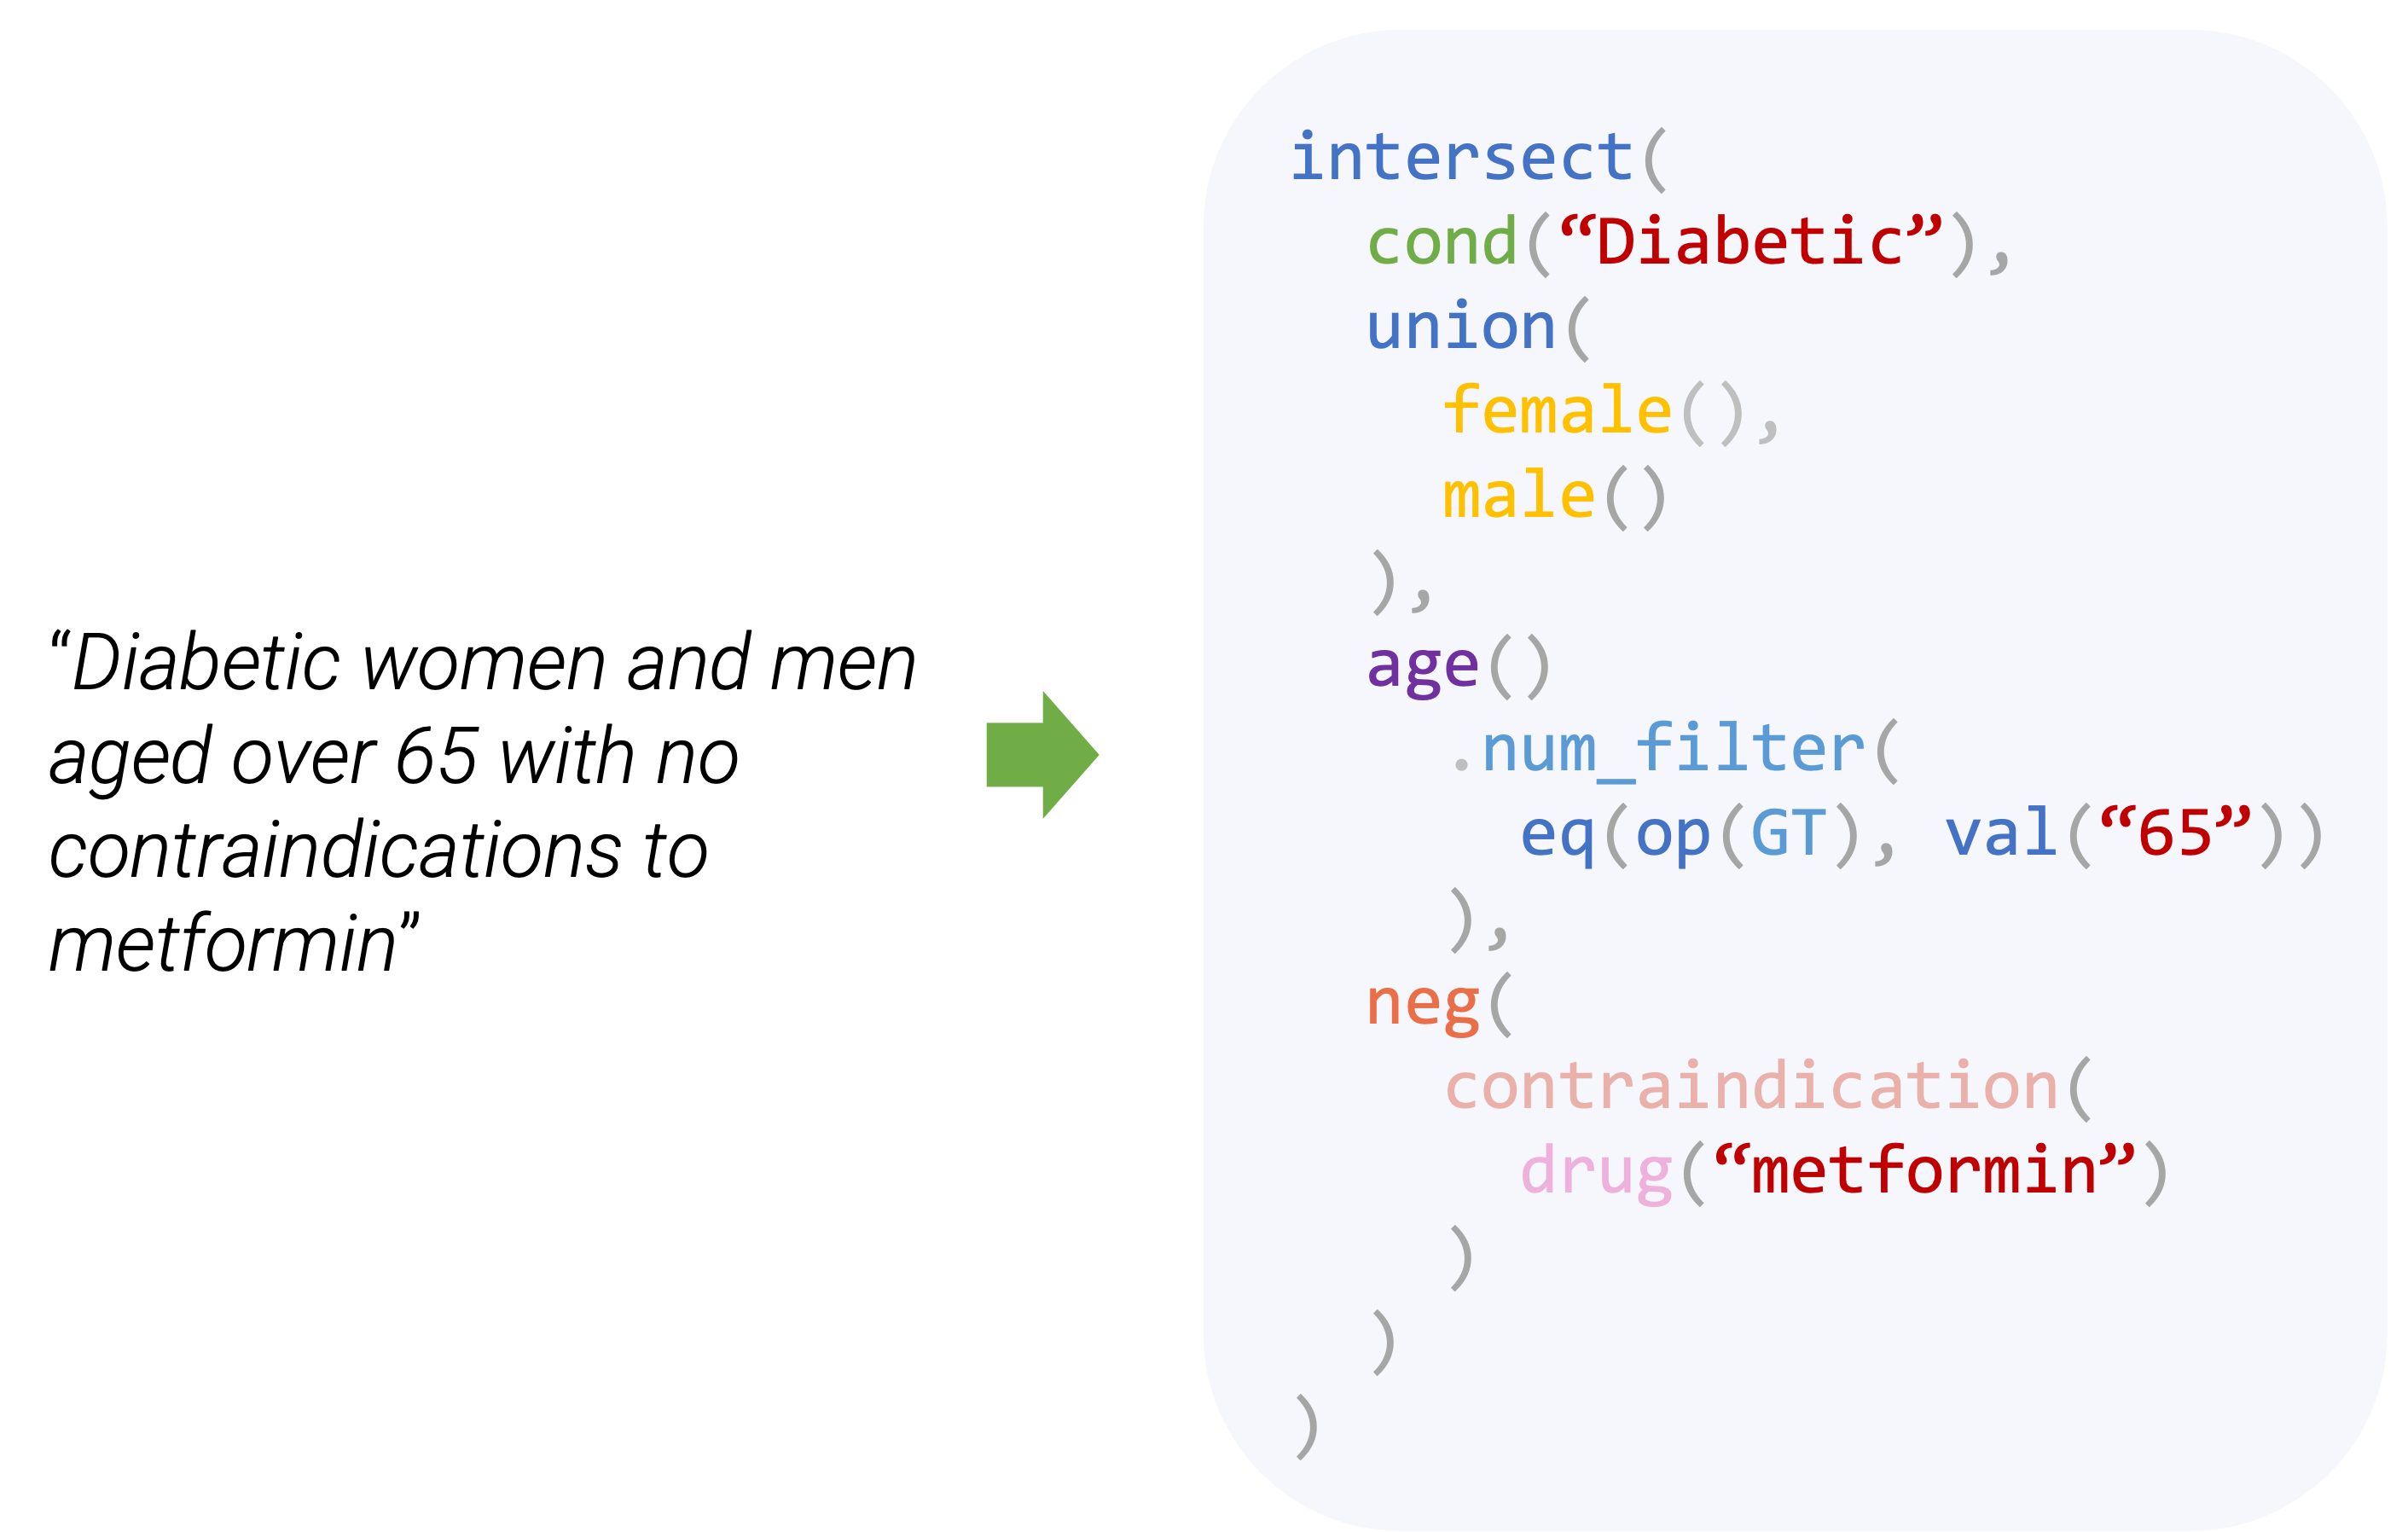
\includegraphics[scale=0.6]{Figures/4_llf_corpus/semantic_parse.png}  
\caption{An example semantic parse using the LLF corpus annotation schema. The hypothetical input sentence is on the left, while the corresponding logical form is shown on the right. Indentations and colors have been added for readability.}
\label{fig_semantic_parse}
\end{figure}

\section{Related Work}

A number of logical (sometimes called "formal") representations of eligibility criteria have been explored by researchers. These include ad hoc expression languages such as EON \cite{musen1996eon}, SAGE \cite{tu2007sage}, ERGO \cite{sim2004ontology}, and EliXR \cite{weng2011elixr}, typically in tree-like dependency structure, Arden Syntax, a prescribed syntax of operators and operations related to health data \cite{hulse1976computerized}, logic-based languages such as Protégé \cite{musen2015protege} and SQL, and others \cite{sordo2004description,miksch1997asbru,o2002chronus}. See Weng \textit{et al} \cite{weng2010formal} for a comprehensive review. As discussed in the previous section, more recent work by Roberts and Demner-Fushman proposed the use of a First Order Logic-based forms \cite{roberts2016annotating} which have been demonstrated to work well in tasks such as question answering \cite{soni2023quehry}.

\section{Methods}

We developed annotation guidelines for the LLF corpus using a simplification of entities and relations from the preceding LCT corpus\cite{dobbins2022leaf}. Generally speaking, LCT \textit{entities} correspond to logical form \textit{functions}, while LCT \textit{relations} correspond to logical form \textit{predicates}. For example, the LCT \textit{Condition} entity has a corresponding \textit{cond()} function, while the \textit{Num-Filter} relation has a corresponding \textit{.num\_filter()} predicate. The LLF annotation guidelines can be found at \url{https://github.com/ndobb/clinical-trials-seq2seq-annotation/wiki}.

We also hypothesized that the performance of predicting logical forms could likely be improved by replacing "raw" tokens in each eligibility criteria with corresponding logical form names derived from named entities from the LCT corpus. For example, given the eligibility criterion: \\

"\textit{Diabetics who smoke}", \\

\noindent we would replace the named entities for "Diabetics" and "smoke": \\ 

\textit{cond("Diabetics") who obs("smoke")} \\

\noindent using \textit{Condition} and \textit{Observation} annotations in the LCT corpus. We call this substituted text an "augmented" eligibility criteria. The augmented criteria syntax reshapes named entities to more closely resemble expected logical form syntax and allows us to leverage the LCT corpus for logical form transformation.

Creation and annotation of the LLF corpus proceeded in the following steps:

\begin{enumerate}
    \item We randomly chose 2,000 lines of eligibility criteria from the LCT corpus, limited to only criteria which included at least one named entity and which were not annotated as hypothetical criteria. 30\% of the 2,000 lines (600) were randomly chosen among lines with particularly complex entity and relation types, such as \textit{If-Then}, \textit{Before-After}, \textit{Contraindication}, etc.
    \item  Each annotation file consists of the text "EXC" if exclusion or "INC" if inclusion (line 1), an original "raw" eligibility criteria (line 3), an augmented eligibility criteria (line 5), and an (initially blank) expected logical form equivalent to annotate (line 7). An example annotation is shown in Figure \ref{fig_annotation_example}.
    \item 3 informatics graduate students met weekly for 2 months to review annotations. Annotators were initially trained on 20 triple-annotated training annotations. 
    \item After training, each annotator was assigned a batch of 100 sentences (one per file) and tasked with writing a logical form version of each.
    \item After each batch was completed, we executed a quality control script to parse each logical form annotation to ensure consistency. Any syntax errors were reported to and corrected by the annotators.
    \item Annotators received additional batches of files to annotate until all 2,000 single-annotated annotations had been completed.
\end{enumerate}

\begin{figure}[h]
  \centering
  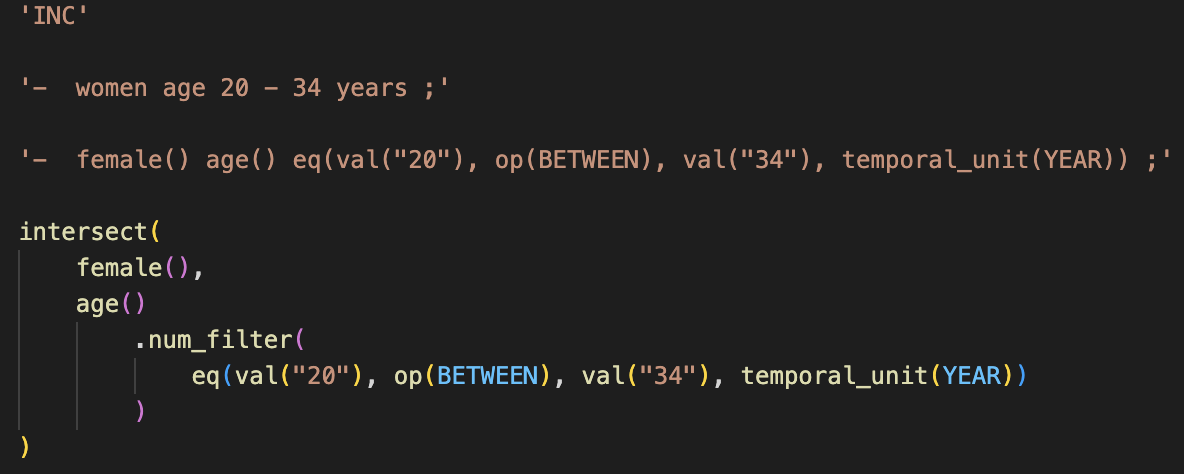
\includegraphics[scale=0.7]{Figures/4_llf_corpus/annotation_example.png}
  \caption{An example LLF corpus annotation. The annotation file is saved in JavaScript (.js) format, which enables syntax highlighting and validation to assist annotators. Whether a given criterion was an inclusion or exclusion criteria is indicated at the top, followed by the original raw text, then augmented text. The final annotated logical forms are shown last.}
  \label{fig_annotation_example}
\end{figure}

The pair-wise mean inter-annotator agreement by BLEU score was 82.4\%. After annotations were completed, we experimented with predicting logical forms by fine-tuning T5 \cite{raffel2020exploring} Seq2Seq models. The T5 architecture and pre-trained models are widely used for and achieve at or near state-of-the-art for many machine translation and semantic parsing tasks. 

Following earlier work on task-oriented dialog semantic parsing structures in the domain of digital assistants, we also experimented using various alternative input-output syntax styles from our original logical forms:

\begin{enumerate}
    \item \textbf{Shift-Reduce}. Einolghozatic \textit{et al.} \cite{einolghozati2019improving} used square brackets instead of parentheses and blank spaces instead of commas. We followed Rongali \textit{et al's} suggestion to add a trailing repeat of function names to improve performance.
    \item \textbf{Pointer}. Rongali \textit{et al.} \cite{rongali2020don} found that replacing input tokens with "$@ptr_{index}$", where \textit{index} corresponds to a token's sequential position in the input text improved performance in their semantic parsing task. We modified this approach by omitting the characters "ptr" and using the sequential position of the quoted span as our index rather than individual token positions.
\end{enumerate}

\section{Results}

We used a randomly sorted 70/20/10 train/test/validation split of the LFF corpus to fine-tune the pretrained T5$_{base}$ model using combinations of these syntax styles. We call our gold standard annotated logical form syntax "Standard" style. Example inputs, outputs, and training results are shown in Table \ref{tbl_llf_corpus}. 

\begin{table}[ht]
    \footnotesize
    \centering
    \def\arraystretch{0.8}
\begin{tabular}{m{2.5cm} m{4.8cm} l l l}
    \toprule
    \textbf{Syntax Style} & \textbf{Example Input} & \textbf{Example Logical Form} & \textbf{BLEU} & \textbf{ROUGE-L} \\
    \midrule
    Raw-text→ Standard       
       & Diabetics who smoke                     
       & $\makecell[cl]{intersect(\\\mathrm{\ \ \ }cond("Diabetics"), \\\mathrm{\ \ \ }obs("smoke")\\)}$
       & 78.7
       & 79.1 \\
    \midrule
    Standard  
       & cond("Diabetics") who obs("smoke")           
       & $\makecell[cl]{intersect(\\\mathrm{\ \ \ }cond("Diabetics"), \\\mathrm{\ \ \ }obs("smoke")\\)}$
       & \textbf{93.5}
       & \textbf{92.3} \\
    \midrule
    Standard+ Pointer
       & cond(@1) who obs(@2)                          
       & $\makecell[cl]{intersect(\\\mathrm{\ \ \ }cond(@1), \\\mathrm{\ \ \ }obs(@2)\\)}$
       & 93.3
       & 91.2 \\
    \midrule
    Shift-Reduce              
       & [cond "Diabetics" cond] who [obs "smoke" obs] 
       & $\makecell[cl]{[intersect\\\mathrm{\ \ \ }[cond\mathrm{\ }"Diabetics"\mathrm{\ }cond]\\\mathrm{\ \ \ }[obs\mathrm{\ }"smoke"\mathrm{\ }obs]\\ intersect]}$
       & 89.8
       & 91.7 \\
    \midrule
    Shift-Reduce+ Pointer     
       & [cond @1 cond] who [obs @2 obs]               
       & $\makecell[cl]{[intersect\\\mathrm{\ \ \ }[cond\mathrm{\ }@1\mathrm{\ }cond]\\\mathrm{\ \ \ }[obs\mathrm{\ }@2\mathrm{\ }obs]\\ intersect]}$
       & 89.4
       & 90.4 \\
    \bottomrule       
\end{tabular}
    \caption{Example inputs and logical form syntax styles with fine-tuning performance results using the T5$_{base}$ model.}
    \label{tbl_llf_corpus}
\end{table} 

We found that our Standard logical forms achieved the highest performance using both BLEU \cite{lin2004rouge} and ROUGE-L \cite{callison2006re} scores, two commonly used metrics in measuring Seq2Seq performance. Replacing raw tokens with function names corresponding to named entities also significantly improved performance (+14.7\%, comparing raw text to Standard input styles), demonstrating that leveraging the LCT corpus to generate augmented text achieved relatively high performance ($>$ 93\% BLEU score) for this task. As it was the highest-performing syntax style and also the most straightforward to parse, we chose to use the Standard logical form style as our IR for this project.

\section{Summary}
We created the LLF corpus, a gold standard human-annotated corpus of 2,000 eligibility criteria and corresponding logical forms. The LLF syntax was developed based on study of past work and entities and relations present in the LCT corpus. Our best performing prediction method using a fine-tuned T5 model achieved $>$ 93\% BLEU score.

\end{document}